\documentclass[12pt]{article}

%packages
%\usepackage{latexsym}
\usepackage{graphicx}
\usepackage{color}
\usepackage{amsmath}
\usepackage{dsfont}
\usepackage{placeins}
\usepackage{amssymb}
\usepackage{wasysym}
\usepackage{abstract}
\usepackage{hyperref}
\usepackage{etoolbox}
\usepackage{datetime}
\usepackage{xcolor}
\usepackage{alphalph}
\usepackage{bm}
\settimeformat{ampmtime}

%\usepackage{pstricks,pst-node,pst-tree}

%\usepackage{algpseudocode}
%\usepackage{amsthm}
%\usepackage{hyperref}
%\usepackage{mathrsfs}
%\usepackage{amsfonts}
%\usepackage{bbding}
%\usepackage{listings}
%\usepackage{appendix}
\usepackage[margin=1in]{geometry}
%\geometry{papersize={8.5in,11in},total={6.5in,9in}}
%\usepackage{cancel}
%\usepackage{algorithmic, algorithm}

\makeatletter
\def\maxwidth{ %
  \ifdim\Gin@nat@width>\linewidth
    \linewidth
  \else
    \Gin@nat@width
  \fi
}
\makeatother

\definecolor{fgcolor}{rgb}{0.345, 0.345, 0.345}
\newcommand{\hlnum}[1]{\textcolor[rgb]{0.686,0.059,0.569}{#1}}%
\newcommand{\hlstr}[1]{\textcolor[rgb]{0.192,0.494,0.8}{#1}}%
\newcommand{\hlcom}[1]{\textcolor[rgb]{0.678,0.584,0.686}{\textit{#1}}}%
\newcommand{\hlopt}[1]{\textcolor[rgb]{0,0,0}{#1}}%
\newcommand{\hlstd}[1]{\textcolor[rgb]{0.345,0.345,0.345}{#1}}%
\newcommand{\hlkwa}[1]{\textcolor[rgb]{0.161,0.373,0.58}{\textbf{#1}}}%
\newcommand{\hlkwb}[1]{\textcolor[rgb]{0.69,0.353,0.396}{#1}}%
\newcommand{\hlkwc}[1]{\textcolor[rgb]{0.333,0.667,0.333}{#1}}%
\newcommand{\hlkwd}[1]{\textcolor[rgb]{0.737,0.353,0.396}{\textbf{#1}}}%

\usepackage{framed}
\makeatletter
\newenvironment{kframe}{%
 \def\at@end@of@kframe{}%
 \ifinner\ifhmode%
  \def\at@end@of@kframe{\end{minipage}}%
  \begin{minipage}{\columnwidth}%
 \fi\fi%
 \def\FrameCommand##1{\hskip\@totalleftmargin \hskip-\fboxsep
 \colorbox{shadecolor}{##1}\hskip-\fboxsep
     % There is no \\@totalrightmargin, so:
     \hskip-\linewidth \hskip-\@totalleftmargin \hskip\columnwidth}%
 \MakeFramed {\advance\hsize-\width
   \@totalleftmargin\z@ \linewidth\hsize
   \@setminipage}}%
 {\par\unskip\endMakeFramed%
 \at@end@of@kframe}
\makeatother

\definecolor{shadecolor}{rgb}{.77, .77, .77}
\definecolor{messagecolor}{rgb}{0, 0, 0}
\definecolor{warningcolor}{rgb}{1, 0, 1}
\definecolor{errorcolor}{rgb}{1, 0, 0}
\newenvironment{knitrout}{}{} % an empty environment to be redefined in TeX

\usepackage{alltt}
\usepackage[T1]{fontenc}

\newcommand{\qu}[1]{``#1''}
\newcounter{probnum}
\setcounter{probnum}{1}

%create definition to allow local margin changes
\def\changemargin#1#2{\list{}{\rightmargin#2\leftmargin#1}\item[]}
\let\endchangemargin=\endlist 

%allow equations to span multiple pages
\allowdisplaybreaks

%define colors and color typesetting conveniences
\definecolor{gray}{rgb}{0.5,0.5,0.5}
\definecolor{black}{rgb}{0,0,0}
\definecolor{white}{rgb}{1,1,1}
\definecolor{blue}{rgb}{0.5,0.5,1}
\newcommand{\inblue}[1]{\color{blue}#1 \color{black}}
\definecolor{green}{rgb}{0.133,0.545,0.133}
\newcommand{\ingreen}[1]{\color{green}#1 \color{black}}
\definecolor{yellow}{rgb}{1,1,0}
\newcommand{\inyellow}[1]{\color{yellow}#1 \color{black}}
\definecolor{orange}{rgb}{0.9,0.649,0}
\newcommand{\inorange}[1]{\color{orange}#1 \color{black}}
\definecolor{red}{rgb}{1,0.133,0.133}
\newcommand{\inred}[1]{\color{red}#1 \color{black}}
\definecolor{purple}{rgb}{0.58,0,0.827}
\newcommand{\inpurple}[1]{\color{purple}#1 \color{black}}
\definecolor{backgcode}{rgb}{0.97,0.97,0.8}
\definecolor{Brown}{cmyk}{0,0.81,1,0.60}
\definecolor{OliveGreen}{cmyk}{0.64,0,0.95,0.40}
\definecolor{CadetBlue}{cmyk}{0.62,0.57,0.23,0}

%define new math operators
\DeclareMathOperator*{\argmax}{arg\,max~}
\DeclareMathOperator*{\argmin}{arg\,min~}
\DeclareMathOperator*{\argsup}{arg\,sup~}
\DeclareMathOperator*{\arginf}{arg\,inf~}
\DeclareMathOperator*{\convolution}{\text{\Huge{$\ast$}}}
\newcommand{\infconv}[2]{\convolution^\infty_{#1 = 1} #2}
%true functions

%%%% GENERAL SHORTCUTS

%shortcuts for pure typesetting conveniences
\newcommand{\bv}[1]{\boldsymbol{#1}}

%shortcuts for compound constants
\newcommand{\BetaDistrConst}{\dfrac{\Gamma(\alpha + \beta)}{\Gamma(\alpha)\Gamma(\beta)}}
\newcommand{\NormDistrConst}{\dfrac{1}{\sqrt{2\pi\sigma^2}}}

%shortcuts for conventional symbols
\newcommand{\tsq}{\tau^2}
\newcommand{\tsqh}{\hat{\tau}^2}
\newcommand{\sigsq}{\sigma^2}
\newcommand{\sigsqsq}{\parens{\sigma^2}^2}
\newcommand{\sigsqovern}{\dfrac{\sigsq}{n}}
\newcommand{\tausq}{\tau^2}
\newcommand{\tausqalpha}{\tau^2_\alpha}
\newcommand{\tausqbeta}{\tau^2_\beta}
\newcommand{\tausqsigma}{\tau^2_\sigma}
\newcommand{\betasq}{\beta^2}
\newcommand{\sigsqvec}{\bv{\sigma}^2}
\newcommand{\sigsqhat}{\hat{\sigma}^2}
\newcommand{\sigsqhatmlebayes}{\sigsqhat_{\text{Bayes, MLE}}}
\newcommand{\sigsqhatmle}[1]{\sigsqhat_{#1, \text{MLE}}}
\newcommand{\bSigma}{\bv{\Sigma}}
\newcommand{\bSigmainv}{\bSigma^{-1}}
\newcommand{\thetavec}{\bv{\theta}}
\newcommand{\thetahat}{\hat{\theta}}
\newcommand{\thetahatmle}{\hat{\theta}_{\mathrm{MLE}}}
\newcommand{\thetavechatmle}{\hat{\thetavec}_{\mathrm{MLE}}}
\newcommand{\muhat}{\hat{\mu}}
\newcommand{\musq}{\mu^2}
\newcommand{\muvec}{\bv{\mu}}
\newcommand{\muhatmle}{\muhat_{\text{MLE}}}
\newcommand{\lambdahat}{\hat{\lambda}}
\newcommand{\lambdahatmle}{\lambdahat_{\text{MLE}}}
\newcommand{\etavec}{\bv{\eta}}
\newcommand{\alphavec}{\bv{\alpha}}
\newcommand{\minimaxdec}{\delta^*_{\mathrm{mm}}}
\newcommand{\ybar}{\bar{y}}
\newcommand{\xbar}{\bar{x}}
\newcommand{\Xbar}{\bar{X}}
\newcommand{\phat}{\hat{p}}
\newcommand{\Phat}{\hat{P}}
\newcommand{\Zbar}{\bar{Z}}
\newcommand{\iid}{~{\buildrel iid \over \sim}~}
\newcommand{\inddist}{~{\buildrel ind \over \sim}~}
\newcommand{\approxdist}{~{\buildrel approx \over \sim}~}
\newcommand{\equalsindist}{~{\buildrel d \over =}~}
\newcommand{\loglik}[1]{\ell\parens{#1}}
\newcommand{\thetahatkminone}{\thetahat^{(k-1)}}
\newcommand{\thetahatkplusone}{\thetahat^{(k+1)}}
\newcommand{\thetahatk}{\thetahat^{(k)}}
\newcommand{\half}{\frac{1}{2}}
\newcommand{\third}{\frac{1}{3}}
\newcommand{\twothirds}{\frac{2}{3}}
\newcommand{\fourth}{\frac{1}{4}}
\newcommand{\fifth}{\frac{1}{5}}
\newcommand{\sixth}{\frac{1}{6}}

%shortcuts for vector and matrix notation
\newcommand{\A}{\bv{A}}
\newcommand{\At}{\A^T}
\newcommand{\Ainv}{\inverse{\A}}
\newcommand{\B}{\bv{B}}
\newcommand{\K}{\bv{K}}
\newcommand{\Kt}{\K^T}
\newcommand{\Kinv}{\inverse{K}}
\newcommand{\Kinvt}{(\Kinv)^T}
\newcommand{\M}{\bv{M}}
\newcommand{\Bt}{\B^T}
\newcommand{\Q}{\bv{Q}}
\newcommand{\Qt}{\Q^T}
\newcommand{\R}{\bv{R}}
\newcommand{\Rt}{\R^T}
\newcommand{\Z}{\bv{Z}}
\newcommand{\X}{\bv{X}}
\renewcommand{\H}{\bv{H}}
\newcommand{\Xsub}{\X_{\text{(sub)}}}
\newcommand{\Xsubadj}{\X_{\text{(sub,adj)}}}
\newcommand{\I}{\bv{I}}
\newcommand{\Y}{\bv{Y}}
\newcommand{\sigsqI}{\sigsq\I}
\renewcommand{\P}{\bv{P}}
\newcommand{\Psub}{\P_{\text{(sub)}}}
\newcommand{\Pt}{\P^T}
\newcommand{\Pii}{P_{ii}}
\newcommand{\Pij}{P_{ij}}
\newcommand{\IminP}{(\I-\P)}
\newcommand{\Xt}{\bv{X}^T}
\newcommand{\XtX}{\Xt\X}
\newcommand{\XtXinv}{\parens{\Xt\X}^{-1}}
\newcommand{\XtXinvXt}{\XtXinv\Xt}
\newcommand{\XXtXinvXt}{\X\XtXinvXt}
\newcommand{\x}{\bv{x}}
\renewcommand{\b}{\bv{b}}
\newcommand{\onevec}{\bv{1}}
\newcommand{\oneton}{1, \ldots, n}
\newcommand{\yoneton}{y_1, \ldots, y_n}
\newcommand{\yonetonorder}{y_{(1)}, \ldots, y_{(n)}}
\newcommand{\Yoneton}{Y_1, \ldots, Y_n}
\newcommand{\iinoneton}{i \in \braces{\oneton}}
\newcommand{\onetom}{1, \ldots, m}
\newcommand{\jinonetom}{j \in \braces{\onetom}}
\newcommand{\xoneton}{x_1, \ldots, x_n}
\newcommand{\Xoneton}{X_1, \ldots, X_n}
\newcommand{\xt}{\x^T}
\newcommand{\y}{\bv{y}}
\newcommand{\yt}{\y^T}
\renewcommand{\c}{\bv{c}}
\newcommand{\ct}{\c^T}
\newcommand{\tstar}{\bv{t}^*}
\renewcommand{\u}{\bv{u}}
\renewcommand{\v}{\bv{v}}
\renewcommand{\a}{\bv{a}}
\newcommand{\s}{\bv{s}}
\newcommand{\yadj}{\y_{\text{(adj)}}}
\newcommand{\xjadj}{\x_{j\text{(adj)}}}
\newcommand{\xjadjM}{\x_{j \perp M}}
\newcommand{\yhat}{\hat{\y}}
\newcommand{\yhatsub}{\yhat_{\text{(sub)}}}
\newcommand{\yhatstar}{\yhat^*}
\newcommand{\yhatstarnew}{\yhatstar_{\text{new}}}
\newcommand{\z}{\bv{z}}
\newcommand{\zt}{\z^T}
\newcommand{\bb}{\bv{b}}
\newcommand{\bbt}{\bb^T}
\newcommand{\bbeta}{\bv{\beta}}
\newcommand{\beps}{\bv{\epsilon}}
\newcommand{\bepst}{\beps^T}
\newcommand{\e}{\bv{e}}
\newcommand{\Mofy}{\M(\y)}
\newcommand{\KofAlpha}{K(\alpha)}
\newcommand{\ellset}{\mathcal{L}}
\newcommand{\oneminalph}{1-\alpha}
\newcommand{\SSE}{\text{SSE}}
\newcommand{\SSEsub}{\text{SSE}_{\text{(sub)}}}
\newcommand{\MSE}{\text{MSE}}
\newcommand{\RMSE}{\text{RMSE}}
\newcommand{\SSR}{\text{SSR}}
\newcommand{\SST}{\text{SST}}
\newcommand{\JSest}{\delta_{\text{JS}}(\x)}
\newcommand{\Bayesest}{\delta_{\text{Bayes}}(\x)}
\newcommand{\EmpBayesest}{\delta_{\text{EmpBayes}}(\x)}
\newcommand{\BLUPest}{\delta_{\text{BLUP}}}
\newcommand{\MLEest}[1]{\hat{#1}_{\text{MLE}}}

%shortcuts for Linear Algebra stuff (i.e. vectors and matrices)
\newcommand{\twovec}[2]{\bracks{\begin{array}{c} #1 \\ #2 \end{array}}}
\newcommand{\threevec}[3]{\bracks{\begin{array}{c} #1 \\ #2 \\ #3 \end{array}}}
\newcommand{\fivevec}[5]{\bracks{\begin{array}{c} #1 \\ #2 \\ #3 \\ #4 \\ #5 \end{array}}}
\newcommand{\twobytwomat}[4]{\bracks{\begin{array}{cc} #1 & #2 \\ #3 & #4 \end{array}}}
\newcommand{\threebytwomat}[6]{\bracks{\begin{array}{cc} #1 & #2 \\ #3 & #4 \\ #5 & #6 \end{array}}}

%shortcuts for conventional compound symbols
\newcommand{\thetainthetas}{\theta \in \Theta}
\newcommand{\reals}{\mathbb{R}}
\newcommand{\complexes}{\mathbb{C}}
\newcommand{\rationals}{\mathbb{Q}}
\newcommand{\integers}{\mathbb{Z}}
\newcommand{\naturals}{\mathbb{N}}
\newcommand{\forallninN}{~~\forall n \in \naturals}
\newcommand{\forallxinN}[1]{~~\forall #1 \in \reals}
\newcommand{\matrixdims}[2]{\in \reals^{\,#1 \times #2}}
\newcommand{\inRn}[1]{\in \reals^{\,#1}}
\newcommand{\mathimplies}{\quad\Rightarrow\quad}
\newcommand{\mathlogicequiv}{\quad\Leftrightarrow\quad}
\newcommand{\eqncomment}[1]{\quad \text{(#1)}}
\newcommand{\limitn}{\lim_{n \rightarrow \infty}}
\newcommand{\limitN}{\lim_{N \rightarrow \infty}}
\newcommand{\limitd}{\lim_{d \rightarrow \infty}}
\newcommand{\limitt}{\lim_{t \rightarrow \infty}}
\newcommand{\limitsupn}{\limsup_{n \rightarrow \infty}~}
\newcommand{\limitinfn}{\liminf_{n \rightarrow \infty}~}
\newcommand{\limitk}{\lim_{k \rightarrow \infty}}
\newcommand{\limsupn}{\limsup_{n \rightarrow \infty}}
\newcommand{\limsupk}{\limsup_{k \rightarrow \infty}}
\newcommand{\floor}[1]{\left\lfloor #1 \right\rfloor}
\newcommand{\ceil}[1]{\left\lceil #1 \right\rceil}

%shortcuts for environments
\newcommand{\beqn}{\vspace{-0.25cm}\begin{eqnarray*}}
\newcommand{\eeqn}{\end{eqnarray*}}
\newcommand{\bneqn}{\vspace{-0.25cm}\begin{eqnarray}}
\newcommand{\eneqn}{\end{eqnarray}}

%shortcuts for mini environments
\newcommand{\parens}[1]{\left(#1\right)}
\newcommand{\squared}[1]{\parens{#1}^2}
\newcommand{\tothepow}[2]{\parens{#1}^{#2}}
\newcommand{\prob}[1]{\mathbb{P}\parens{#1}}
\newcommand{\cprob}[2]{\prob{#1~|~#2}}
\newcommand{\littleo}[1]{o\parens{#1}}
\newcommand{\bigo}[1]{O\parens{#1}}
\newcommand{\Lp}[1]{\mathbb{L}^{#1}}
\renewcommand{\arcsin}[1]{\text{arcsin}\parens{#1}}
\newcommand{\prodonen}[2]{\bracks{\prod_{#1=1}^n #2}}
\newcommand{\mysum}[4]{\sum_{#1=#2}^{#3} #4}
\newcommand{\sumonen}[2]{\sum_{#1=1}^n #2}
\newcommand{\infsum}[2]{\sum_{#1=1}^\infty #2}
\newcommand{\infprod}[2]{\prod_{#1=1}^\infty #2}
\newcommand{\infunion}[2]{\bigcup_{#1=1}^\infty #2}
\newcommand{\infinter}[2]{\bigcap_{#1=1}^\infty #2}
\newcommand{\infintegral}[2]{\int^\infty_{-\infty} #2 ~\text{d}#1}
\newcommand{\supthetas}[1]{\sup_{\thetainthetas}\braces{#1}}
\newcommand{\bracks}[1]{\left[#1\right]}
\newcommand{\braces}[1]{\left\{#1\right\}}
\newcommand{\set}[1]{\left\{#1\right\}}
\newcommand{\abss}[1]{\left|#1\right|}
\newcommand{\norm}[1]{\left|\left|#1\right|\right|}
\newcommand{\normsq}[1]{\norm{#1}^2}
\newcommand{\inverse}[1]{\parens{#1}^{-1}}
\newcommand{\rowof}[2]{\parens{#1}_{#2\cdot}}

%shortcuts for functionals
\newcommand{\realcomp}[1]{\text{Re}\bracks{#1}}
\newcommand{\imagcomp}[1]{\text{Im}\bracks{#1}}
\newcommand{\range}[1]{\text{range}\bracks{#1}}
\newcommand{\colsp}[1]{\text{colsp}\bracks{#1}}
\newcommand{\rowsp}[1]{\text{rowsp}\bracks{#1}}
\newcommand{\tr}[1]{\text{tr}\bracks{#1}}
\newcommand{\rank}[1]{\text{rank}\bracks{#1}}
\newcommand{\proj}[2]{\text{Proj}_{#1}\bracks{#2}}
\newcommand{\projcolspX}[1]{\text{Proj}_{\colsp{\X}}\bracks{#1}}
\newcommand{\median}[1]{\text{median}\bracks{#1}}
\newcommand{\mean}[1]{\text{mean}\bracks{#1}}
\newcommand{\dime}[1]{\text{dim}\bracks{#1}}
\renewcommand{\det}[1]{\text{det}\bracks{#1}}
\newcommand{\expe}[1]{\mathbb{E}\bracks{#1}}
\newcommand{\expeabs}[1]{\expe{\abss{#1}}}
\newcommand{\expesub}[2]{\mathbb{E}_{#1}\bracks{#2}}
\newcommand{\indic}[1]{\mathds{1}_{#1}}
\newcommand{\var}[1]{\mathbb{V}\text{ar}\bracks{#1}}
\newcommand{\cov}[2]{\mathbb{C}\text{ov}\bracks{#1, #2}}
\newcommand{\corr}[2]{\text{Corr}\bracks{#1, #2}}
\newcommand{\se}[1]{\mathbb{S}\text{E}\bracks{#1}}
\newcommand{\seest}[1]{\hat{\mathbb{S}\text{E}}\bracks{#1}}
\newcommand{\bias}[1]{\text{Bias}\bracks{#1}}
\newcommand{\derivop}[2]{\dfrac{\text{d}}{\text{d} #1}\bracks{#2}}
\newcommand{\partialop}[2]{\dfrac{\partial}{\partial #1}\bracks{#2}}
\newcommand{\secpartialop}[2]{\dfrac{\partial^2}{\partial #1^2}\bracks{#2}}
\newcommand{\mixpartialop}[3]{\dfrac{\partial^2}{\partial #1 \partial #2}\bracks{#3}}

%shortcuts for functions
\renewcommand{\exp}[1]{\mathrm{exp}\parens{#1}}
\renewcommand{\cos}[1]{\text{cos}\parens{#1}}
\renewcommand{\sin}[1]{\text{sin}\parens{#1}}
\newcommand{\sign}[1]{\text{sign}\parens{#1}}
\newcommand{\are}[1]{\mathrm{ARE}\parens{#1}}
\newcommand{\natlog}[1]{\ln\parens{#1}}
\newcommand{\oneover}[1]{\frac{1}{#1}}
\newcommand{\overtwo}[1]{\frac{#1}{2}}
\newcommand{\overn}[1]{\frac{#1}{n}}
\newcommand{\oneoversqrt}[1]{\oneover{\sqrt{#1}}}
\newcommand{\sqd}[1]{\parens{#1}^2}
\newcommand{\loss}[1]{\ell\parens{\theta, #1}}
\newcommand{\losstwo}[2]{\ell\parens{#1, #2}}
\newcommand{\cf}{\phi(t)}

%English language specific shortcuts
\newcommand{\ie}{\textit{i.e.} }
\newcommand{\AKA}{\textit{AKA} }
\renewcommand{\iff}{\textit{iff}}
\newcommand{\eg}{\textit{e.g.} }
\newcommand{\st}{\textit{s.t.} }
\newcommand{\wrt}{\textit{w.r.t.} }
\newcommand{\mathst}{~~\text{\st}~~}
\newcommand{\mathand}{~~\text{and}~~}
\newcommand{\ala}{\textit{a la} }
\newcommand{\ppp}{posterior predictive p-value}
\newcommand{\dd}{dataset-to-dataset}

%shortcuts for distribution titles
\newcommand{\logistic}[2]{\mathrm{Logistic}\parens{#1,\,#2}}
\newcommand{\bernoulli}[1]{\mathrm{Bernoulli}\parens{#1}}
\newcommand{\betanot}[2]{\mathrm{Beta}\parens{#1,\,#2}}
\newcommand{\stdbetanot}{\betanot{\alpha}{\beta}}
\newcommand{\multnormnot}[3]{\mathcal{N}_{#1}\parens{#2,\,#3}}
\newcommand{\normnot}[2]{\mathcal{N}\parens{#1,\,#2}}
\newcommand{\classicnormnot}{\normnot{\mu}{\sigsq}}
\newcommand{\stdnormnot}{\normnot{0}{1}}
\newcommand{\uniformdiscrete}[1]{\mathrm{Uniform}\parens{\braces{#1}}}
\newcommand{\uniform}[2]{\mathrm{U}\parens{#1,\,#2}}
\newcommand{\stduniform}{\uniform{0}{1}}
\newcommand{\geometric}[1]{\mathrm{Geometric}\parens{#1}}
\newcommand{\hypergeometric}[3]{\mathrm{Hypergeometric}\parens{#1,\,#2,\,#3}}
\newcommand{\exponential}[1]{\mathrm{Exp}\parens{#1}}
\newcommand{\gammadist}[2]{\mathrm{Gamma}\parens{#1, #2}}
\newcommand{\poisson}[1]{\mathrm{Poisson}\parens{#1}}
\newcommand{\binomial}[2]{\mathrm{Binomial}\parens{#1,\,#2}}
\newcommand{\negbin}[2]{\mathrm{NegBin}\parens{#1,\,#2}}
\newcommand{\rayleigh}[1]{\mathrm{Rayleigh}\parens{#1}}
\newcommand{\multinomial}[2]{\mathrm{Multinomial}\parens{#1,\,#2}}
\newcommand{\gammanot}[2]{\mathrm{Gamma}\parens{#1,\,#2}}
\newcommand{\cauchynot}[2]{\text{Cauchy}\parens{#1,\,#2}}
\newcommand{\invchisqnot}[1]{\text{Inv}\chisq{#1}}
\newcommand{\invscaledchisqnot}[2]{\text{ScaledInv}\ncchisq{#1}{#2}}
\newcommand{\invgammanot}[2]{\text{InvGamma}\parens{#1,\,#2}}
\newcommand{\chisq}[1]{\chi^2_{#1}}
\newcommand{\ncchisq}[2]{\chi^2_{#1}\parens{#2}}
\newcommand{\ncF}[3]{F_{#1,#2}\parens{#3}}

%shortcuts for PDF's of common distributions
\newcommand{\logisticpdf}[3]{\oneover{#3}\dfrac{\exp{-\dfrac{#1 - #2}{#3}}}{\parens{1+\exp{-\dfrac{#1 - #2}{#3}}}^2}}
\newcommand{\betapdf}[3]{\dfrac{\Gamma(#2 + #3)}{\Gamma(#2)\Gamma(#3)}#1^{#2-1} (1-#1)^{#3-1}}
\newcommand{\normpdf}[3]{\frac{1}{\sqrt{2\pi#3}}\exp{-\frac{1}{2#3}(#1 - #2)^2}}
\newcommand{\normpdfvarone}[2]{\dfrac{1}{\sqrt{2\pi}}e^{-\half(#1 - #2)^2}}
\newcommand{\chisqpdf}[2]{\dfrac{1}{2^{#2/2}\Gamma(#2/2)}\; {#1}^{#2/2-1} e^{-#1/2}}
\newcommand{\invchisqpdf}[2]{\dfrac{2^{-\overtwo{#1}}}{\Gamma(#2/2)}\,{#1}^{-\overtwo{#2}-1}  e^{-\oneover{2 #1}}}
\newcommand{\exponentialpdf}[2]{#2\exp{-#2#1}}
\newcommand{\poissonpdf}[2]{\dfrac{e^{-#1} #1^{#2}}{#2!}}
\newcommand{\binomialpdf}[3]{\binom{#2}{#1}#3^{#1}(1-#3)^{#2-#1}}
\newcommand{\rayleighpdf}[2]{\dfrac{#1}{#2^2}\exp{-\dfrac{#1^2}{2 #2^2}}}
\newcommand{\gammapdf}[3]{\dfrac{#3^#2}{\Gamma\parens{#2}}#1^{#2-1}\exp{-#3 #1}}
\newcommand{\cauchypdf}[3]{\oneover{\pi} \dfrac{#3}{\parens{#1-#2}^2 + #3^2}}
\newcommand{\Gammaf}[1]{\Gamma\parens{#1}}

%shortcuts for miscellaneous typesetting conveniences
\newcommand{\notesref}[1]{\marginpar{\color{gray}\tt #1\color{black}}}

%%%% DOMAIN-SPECIFIC SHORTCUTS

%Real analysis related shortcuts
\newcommand{\zeroonecl}{\bracks{0,1}}
\newcommand{\forallepsgrzero}{\forall \epsilon > 0~~}
\newcommand{\lessthaneps}{< \epsilon}
\newcommand{\fraccomp}[1]{\text{frac}\bracks{#1}}

%Bayesian related shortcuts
\newcommand{\yrep}{y^{\text{rep}}}
\newcommand{\yrepisq}{(\yrep_i)^2}
\newcommand{\yrepvec}{\bv{y}^{\text{rep}}}


%Probability shortcuts
\newcommand{\SigField}{\mathcal{F}}
\newcommand{\ProbMap}{\mathcal{P}}
\newcommand{\probtrinity}{\parens{\Omega, \SigField, \ProbMap}}
\newcommand{\convp}{~{\buildrel p \over \rightarrow}~}
\newcommand{\convLp}[1]{~{\buildrel \Lp{#1} \over \rightarrow}~}
\newcommand{\nconvp}{~{\buildrel p \over \nrightarrow}~}
\newcommand{\convae}{~{\buildrel a.e. \over \longrightarrow}~}
\newcommand{\convau}{~{\buildrel a.u. \over \longrightarrow}~}
\newcommand{\nconvau}{~{\buildrel a.u. \over \nrightarrow}~}
\newcommand{\nconvae}{~{\buildrel a.e. \over \nrightarrow}~}
\newcommand{\convd}{~{\buildrel \mathcal{D} \over \rightarrow}~}
\newcommand{\nconvd}{~{\buildrel \mathcal{D} \over \nrightarrow}~}
\newcommand{\withprob}{~~\text{w.p.}~~}
\newcommand{\io}{~~\text{i.o.}}

\newcommand{\Acl}{\bar{A}}
\newcommand{\ENcl}{\bar{E}_N}
\newcommand{\diam}[1]{\text{diam}\parens{#1}}

\newcommand{\taua}{\tau_a}

\newcommand{\myint}[4]{\int_{#2}^{#3} #4 \,\text{d}#1}
\newcommand{\laplacet}[1]{\mathscr{L}\bracks{#1}}
\newcommand{\laplaceinvt}[1]{\mathscr{L}^{-1}\bracks{#1}}
\renewcommand{\min}[1]{\text{min}\braces{#1}}
\renewcommand{\max}[1]{\text{max}\braces{#1}}

\newcommand{\Vbar}[1]{\bar{V}\parens{#1}}
\newcommand{\expnegrtau}{\exp{-r\tau}}

%%% problem typesetting
\definecolor{darkgrey}{rgb}{0.10,0.10,0.9}

\newcommand{\problem}[1]{\noindent \colorbox{black}{{\color{yellow} \large{\textsf{\textbf{Problem \arabic{probnum}}}}~}} \addtocounter{probnum}{1} \vspace{0.2cm} \\ \iftoggle{professormode}{}{\color{darkgrey}} #1}

\newcommand{\easysubproblem}[1]{\ingreen{\item} \iftoggle{professormode}{}{\color{darkgrey}} [easy] #1 \color{black} }
\newcommand{\intermediatesubproblem}[1]{\inorange{\item} \iftoggle{professormode}{}{\color{darkgrey}} [harder] #1 \color{black} }
\newcommand{\hardsubproblem}[1]{\inred{\item} \iftoggle{professormode}{}{\color{darkgrey}} [difficult] #1 \color{black} }
\newcommand{\extracreditsubproblem}[1]{\inpurple{\item} \iftoggle{professormode}{}{\color{darkgrey}} [E.C.] #1 \color{black} }


\newcommand{\spc}[1]{\iftoggle{professormode}{\\ \vspace{#1cm}}{\\ \vspace{-0.3cm}}}

\makeatletter
\newalphalph{\alphmult}[mult]{\@alph}{26}
\renewcommand{\labelenumi}{(\alphmult{\value{enumi}})}

\newcommand{\support}[1]{\text{Supp}\bracks{#1}}
\newcommand{\mode}[1]{\text{Mode}\bracks{#1}}
\newcommand{\IQR}[1]{\text{IQR}\bracks{#1}}
\newcommand{\quantile}[2]{\text{Quantile}\bracks{#1,\,#2}}


\newtoggle{professormode}
%\toggletrue{professormode} %STUDENTS: DELETE or COMMENT this line



\title{MATH 342W / 642 / RM 742 Spring \the\year~ HW \#5}

\author{Sergio E. Garcia Tapia} %STUDENTS: write your name here

\iftoggle{professormode}{
\date{Due 6PM May 16 \\ \vspace{0.5cm} \small (this document last updated \currenttime~on \today)}
}

\renewcommand{\abstractname}{Instructions and Philosophy}

\begin{document}
\maketitle

\iftoggle{professormode}{
\begin{abstract}
The path to success in this class is to do many problems. Unlike other courses, exclusively doing reading(s) will not help. Coming to lecture is akin to watching workout videos; thinking about and solving problems on your own is the actual ``working out.''  Feel free to \qu{work out} with others; \textbf{I want you to work on this in groups.}

Reading is still \textit{required}. You should be googling and reading about all the concepts introduced in class online. This is your responsibility to supplement in-class with your own readings.

The problems below are color coded: \ingreen{green} problems are considered \textit{easy} and marked \qu{[easy]}; \inorange{yellow} problems are considered \textit{intermediate} and marked \qu{[harder]}, \inred{red} problems are considered \textit{difficult} and marked \qu{[difficult]} and \inpurple{purple} problems are extra credit. The \textit{easy} problems are intended to be ``giveaways'' if you went to class. Do as much as you can of the others; I expect you to at least attempt the \textit{difficult} problems. 

This homework is worth 100 points but the point distribution will not be determined until after the due date. See syllabus for the policy on late homework.

Up to 7 points are given as a bonus if the homework is typed using \LaTeX. Links to instaling \LaTeX~and program for compiling \LaTeX~is found on the syllabus. You are encouraged to use \url{overleaf.com}. If you are handing in homework this way, read the comments in the code; there are two lines to comment out and you should replace my name with yours and write your section. The easiest way to use overleaf is to copy the raw text from hwxx.tex and preamble.tex into two new overleaf tex files with the same name. If you are asked to make drawings, you can take a picture of your handwritten drawing and insert them as figures or leave space using the \qu{$\backslash$vspace} command and draw them in after printing or attach them stapled.

The document is available with spaces for you to write your answers. If not using \LaTeX, print this document and write in your answers. I do not accept homeworks which are \textit{not} on this printout. Keep this first page printed for your records.

\end{abstract}

\thispagestyle{empty}
\vspace{1cm}
NAME: \line(1,0){380}
\clearpage
}




\problem{These are some questions related to probability estimation modeling and asymmetric cost modeling. It might be helpful to look back to the review the logistic regression  before doing this problem.}

\begin{enumerate}

\easysubproblem{Graph a canonical ROC and label the axes. In your drawing estimate AUC. Explain very clearly what is measured by the $x$ axis and the $y$ axis.}\spc{7}

See the following figure:

\begin{center}
	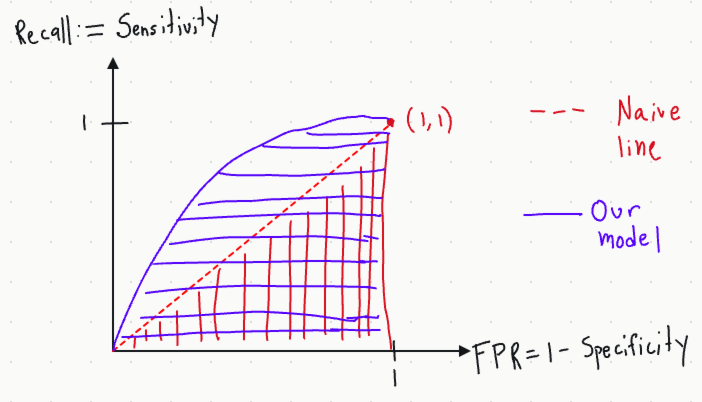
\includegraphics[width=0.6\textwidth]{exercise-01-a-roc}
\end{center}

In the plot, the $x$-axis is the \textit{False Positive Rate} ($FPR$),
which is given by

\begin{align*}
	FPR := \frac{FP}{N}
\end{align*}

where $FP$ is the number of false positive predictions by a classification model
and $N$ is the total number of ``negative" (0) responses in the phenomenon under
consideration. The $FPR$ answers the question, ``of the values our model predicts
as negative, what proportion are incorrect?" The $y$-axis corresponds to
\textit{Recall}, given by
\begin{align*}
	\text{Recall} := \frac{TP}{P}
\end{align*}

Recall answers the question ``what proportion of the positive responses did
we successfully predict correctly?". Each point on the ROC curve is a $(FPR, \text{Recall})$
pair, and each value of that pair is a function of $p_{\text{th}}$, the probability
threshold used for prediction. Therefore, the curve actually shows several
binary classification models for a given probability estimation model (one for
each value fo $p_{th}$).

In the plot, the dotted (red) line represents a
naive model, which corresponds to probability predictions made by picking
values from a uniform distribution on $(0, 1)$. The area under the curve (AUC) for the
naive model is 0.5. In purple with a solid line is ``our model", which
we are assuming outperforms the naive model. The area under the curve is
probably around 0.75.

\easysubproblem{Pick one point on your ROC curve from the previous question. Explain a situation why you would employ this model.}\spc{3}

See the following figure:

\begin{center}
	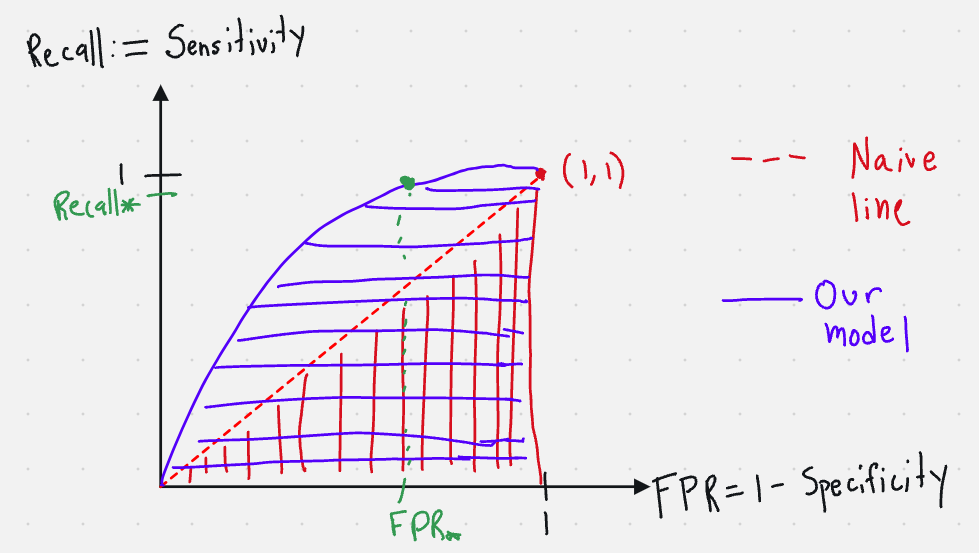
\includegraphics[width=0.6\textwidth]{exercise-01-b-roc}
\end{center}

I picked a point $(FPR_*, \text{Recall}_*)$, which corresponds to a model
built with some $p_{\text{th}_*}$ value that exhibits high Recall,
and relatively high $FPR$. A high Recall model implicitly weighs false
negatives as more costly. Imagine designing a fire alarm system that
attempts to detect whether there is a fire in a building. A false positive
means the alarm goes off and the firefighters are called in, but there
is no actual fire. A false negative means the alarm does not detect
a fire, but there is in fact a fire. In this case false negatives
are more costly because human lives are at stake.

\intermediatesubproblem{Graph a FDR-FOR curve and label the axes. Explain very clearly what is measured by the $x$ axis and the $y$ axis.}\spc{7}

See the following figure:

\begin{center}
	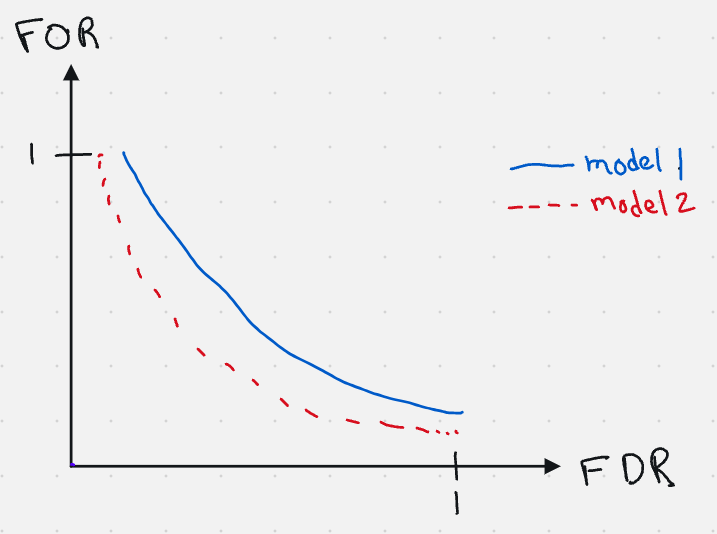
\includegraphics[width=0.5\textwidth]{exercise-01-c-fdr-for}
\end{center}

In the plot, the $x$-axis is the \textit{False Discovery Rate}, given by

\begin{align*}
	FDR := \frac{FP}{PP}
\end{align*}

where $FP$ is the number of false positives and $PP$ is the number of predicted
positives. $FDR$ measures the rate of mistakes in the positive predictions.
In the $y$-axis is the \textit{False Omission Rate}, given by

\begin{align*}
	FOR := \frac{FN}{PN}
\end{align*}

where $FN$ is the number of false negatives and $PN$ is the number of predicted
negatives.  $FOR$ measures the rate of mistakes in the negative predictions.
Each point on the $FDR$-$FOR$ curve corresponds to a different $p_{\text{th}}$
value, th e probability threshold used for prediction. The plot shows two curves.
and each curve corresponds to a single probability estimation model, but several binary
classification models (one for each value of $p_{\text{th}}$). The curves
show that there is a trade-off between $FDR$ and $FOR$. As $p_{\text{th}}$
increases, $FDR$ decreases while $FOR$ increases.

\easysubproblem{Pick one point on your FDR-FOR curve from the previous question. Explain a situation why you would employ this model.}\spc{3}

See the following figure:

\begin{center}
	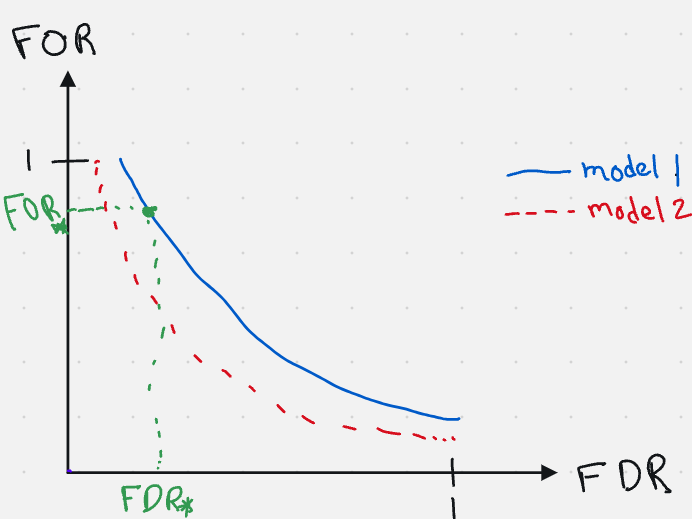
\includegraphics[width=0.5\textwidth]{exercise-01-d-fdr-for}
\end{center}

I picked a point corresponding to a high $FOR$ and a low $FDR$. This might make sense
in a situation where the cost of false positives is prohibitive in comparison with
the cost of false negatives. Suppose, for example, a secured facility that
uses biometric information to determine whether to allow a person to enter.
A false positive in this situation means letting uncleared personnel enter the
facility, while a false negative may be an inconvenience to someone who actually
works there but can be resolved. The cost of false positives is high because
it puts the security of the facility at risk.

\hardsubproblem{[MA] The line of random guessing on the ROC curve is the diagonal line with slope one extending from the origin. What is the corresponding line of random guessing in the FDR-FOR curve? This is not easy...}\spc{5}
\end{enumerate}



\problem{These are some questions related to bias-variance decomposition. Assume the two assumptions from the notes about the random variable model that produces the $\delta$ values, the error due to ignorance.}

\begin{enumerate}
\easysubproblem{Write down (do not derive) the decomposition of MSE for a given $\x_*$ where $\mathbb{D}$ is assumed fixed but the response associated with $\x_*$ is assumed random.}\spc{1}

The $MSE$ for a given $\bm{x}_*$ where the response associated with
$\bm{x}_*$ is random but $\mathbb{D}$ is not random is given by

\begin{align*}
	MSE(\bm{x}_*) = \sigma^2 + (\text{Bias}[\bm{x}_*])^2
\end{align*}

Here, $\sigma^2 = \text{Var}[\Delta \mid \bm{x}]$ for all $\bm{x}$ by one of our
assumptions (homoskedasticity). $\Delta$ is a random variable from which the ignorance
errors are realized. Also, the bias is given by

\begin{align*}
	\text{Bias}[\bm{x}_*] = f(\bm{x}_*) - g(\bm{x}_*)
\end{align*}

where $f$ is the conditional expectation function for the phenomenon in question,
and $g$ is a function from some candidate set $\mathcal{H}$ output by an algorithm
attempting to fit $f$. In fact, $\text{Bias}[\bm{x}_*] := \mathbb{E}[E_* \mid \bm{x}_*]$
and $MSE[\bm{x}_*] = \mathbb{E}[E_*^2 \mid \bm{x}_*]$, but using our assumptions
these are shown to be the expressions presented earlier. $E_*$ is a random variable
from which residuals are realized, defined as $E_* := Y_* - g(\bm{x}_*)$.

\easysubproblem{Write down (do not derive) the decomposition of MSE for a given $\x_*$ where the responses in $\mathbb{D}$ is random but the $\X$ matrix is assumed fixed and the response associated with $\x_*$ is assumed random like previously.}\spc{3}

This time, we have

\begin{align*}
	\text{MSE}[\bm{x}_*] = \sigma^2 + (\text{Bias}[G(\bm{x}_*)])^2 + \text{Var}[G(\bm{x}_*)]
\end{align*}

Here, $G=\mathcal{A}(\mathbb{D}, \mathcal{H})$, and it is a random variable
because the responses are random. That is, the randomness in $\Delta_1,\ldots,\Delta_n$
make it so that we have random $Y_1,\ldots,Y_n$, and in turn our prediction function $G$
is derived from a random $G$.

\easysubproblem{Write down (do not derive) the decomposition of MSE for general predictions of a phenomenon where all quantities are considered random.}\spc{3}

\begin{align*}
	\text{MSE} := \mathbb{E}[\text{MSE}[\bm{x}_*]] = \sigma^2 + \mathbb{E}_X[(\text{Bias}[G(\bm{x}_*)])^2] + \mathbb{E}_X[\text{Var}[G(\bm{x}_*)]]
\end{align*}

\hardsubproblem{Why is it in (a) there is only a \qu{bias} but no \qu{variance} term? Why did the additional source of randomness in (b) spawn the variance term, a new source of error?}\spc{6}

Recall the MSE is defined as

\begin{align*}
	\text{MSE}[\bm{x}_*] = \mathbb{E}[(Y_* - g(\bm{x}_*))^2]
\end{align*}

In (a), since none of the data in $\mathbb{D}$ is random, the prediction function
$g$ is deterministic (i.e., not random) as a function of $\bm{x}_*$,
and similarly $f$ is also. Therefore, in the computation of the MSE as defined
above, $g$ comes out of the expectation, and no variance term survives.
Put another way, since there is no randomness in any component of $\mathbb{D}$
(i.e. neither the responses nor the features), the $g$ is the same each time.

In (b), once we allow randomness in the responses, this in turn makes the
prediction function nondeterministic, meaning it makes our prediction
function $g$ into a random variable $G$. The randomness in the responses
in $\mathbb{D}$ leads to construction of different $g$'s.
Therefore for any given point $\bm{x}_*$, our predictions vary depending on what
realization of $G$ that we use, and this variability is captured by the variance
term.

\intermediatesubproblem{A high bias / low variance algorithm is underfit or overfit?}\spc{-0.5}

Bias is a measure of underfitting or misspecification error,
and variance is a measure of overfitting or estimation error. Since
bias is high, underfit errror is high, and since variance is low, overfit
error is low. Hence, overall we get underfitting.

\intermediatesubproblem{A low bias / high variance algorithm is underfit or overfit?}\spc{-0.5}

Similar to before, low bias means there is little underfitting error,
and high variance means large estimation error (and hence high overfitting error)
(for example we are using junk features). Overall, we have a high overfitting error.

\intermediatesubproblem{Explain why bagging reduces MSE for \qu{free} regardless of the algorithm employed.}\spc{6}

When bagging, we ship as our prediction function the average of $M$ prediction
functions

\begin{align*}
	g_{\text{avg}} := \frac{1}{M} \sum_{m=1}^{M} g_m
\end{align*}

Bagging is done such that the $g_m$ become somewhat decoupled, and this
leads to a reduction in the covariance among them. In turn, the covariance
reduces the variance term in the MSE, and hence the MSE also reduces.

\intermediatesubproblem{Explain why RF reduces MSE atop bagging $M$ trees and specifically mention the target that it attacks in the MSE decomposition formula and why it's able to reduce that target.}\spc{5}

Random forests use a subset of the features when building trees rather than all
of the features. Therefore the models are built based on different subsets of
features, further decoupling them. The result is a reduction in the covariance,
and hence of the variance term and overall MSE.

\hardsubproblem{When can RF lose to bagging $M$ trees? Hint: think hyperparameter choice.}\spc{5}

It can lose for poor choices of the $m_{\text{try}}$ hyperparameter.
For example, if $m_{\text{try}} = 1$, then each tree built is likely to
underfit heavily. As $m_{\text{try}}$ increases, the number of possible
subsets of features increases, so there are more options for the different
trees, while allowing enough degrees of freedom for a better fit.

\end{enumerate}



%\problem{These are some questions related to correlation-causation and interpretation of OLS coefficients.}
%
%\begin{enumerate}
%\easysubproblem{Consider a fitted OLS model for y with features $x_1$, $x_2$, \ldots, $x_p$. Provide the most correct interpretation of the quantity $b_1$ you can.}\spc{6}
%
%
%\easysubproblem{If $x$ and $y$ are correlated but their relationship isn't causal, draw a diagram below that includes $z$.}\spc{6}
%
%\easysubproblem{To show that $x$ is causal for $y$, what specifically has to be demonstrated? Answer with a couple of sentences.}\spc{4}
%
%\intermediatesubproblem{If we fit a model for y using $x_1$, $x_2$, \ldots, $x_7$, provide an example real-world illustration of the causal diagram for $y$ including the $z_1$, $z_2$, $z_3$.}\spc{5}
%
%
%\end{enumerate}
%
%
\problem{These are some questions related to missingness.}

\begin{enumerate}
\easysubproblem{[MA] What are the three missing data mechanisms? Provide an example when each occurs (i.e., a real world situation). We didn't really cover this in class so I'm making it a MA question only. This concept will NOT be on the exam.}\spc{3}

\easysubproblem{Why is listwise-deletion a \textit{terrible} idea to employ in your $\mathbb{D}$ when doing supervised learning?}\spc{3}

You risk suffering from sampling bias. For example if your data set has an age
feature, and the observations where age is larger (older) shows a lot of missingness,
dropping them means that that population is not represented in the model.
When we go off to predict, our model will extrapolate poorly.

\easysubproblem{Why is it good practice to augment $\mathbb{D}$ to include missingness dummies? In other words, why would this increase oos predictive accuracy?}\spc{4}

When some features are missing for a given observation, that missingness may be related
to the missingness of other features. Moreover, it's possible that the missingness
itself tells us important information about the individual. For example,
for a student that is absent from school a lot, the lack of academic records
may be as the actual grades they would have had if the grade were present.
Thus the model is better equipped to predict out-of-sample.

\easysubproblem{To impute missing values in $\mathbb{D}$, what is a good default strategy and why?}\spc{3}

A good default strategy is to assume that data is not missing at random and to
construct a matrix $M$ of the missing values. That is,
the columns of $M$ correspond to columns of $X$ that exhibit missingness.
If $X$ is $n\times p$, then $M$ is $n\times q$ for some $q\leq p$. Entry
$M_{ij}$ is $1$ is the $i$th unit has missingness for some feature in $X$
index $j$ (not the $j$th feature of $X$, but the $j$th feature missing
in $X$). Then, we compute an imputed matrix by applying an imputation algorithm
on the augmented matrix:

\begin{align*}
	[X_{\text{imp}} \mid M] = \text{Impute}([X \mid M], \bm{y})
\end{align*}

The reason it is a good idea is that data is likely not missing at random;
we simply do not know why it is missing. Moreover, the missingness may
tell us something about the units themselves, so this can lead to better
predictive value.

\end{enumerate}
%
%\problem{These are some questions related to lasso, ridge and the elastic net.}
%
%\begin{enumerate}
%\easysubproblem{Write down the objective function to be minimized for ridge. Use $\lambda$ as the hyperparameter.}\spc{2}
%
%\easysubproblem{Write down the objective function to be minimized for lasso. Use $\lambda$ as the hyperparameter.}\spc{3}
%
%\easysubproblem{We spoke in class about when ridge and lasso are employed. Based on this discussion, why should we restrict $\lambda > 0$?}\spc{3}
%
%\intermediatesubproblem{Why is lasso sometimes used a preprocessing step to remove variables that likely are not important in predicting the response?}\spc{3}
%
%
%\easysubproblem{Assume $\X$ is orthonormal. One can derive $\b_{\text{lasso}}$ in closed form. Copy the answer from the wikipedia page. Compare $\b_{\text{lasso}}$ to $\b_{\text{OLS}}$.}\spc{8}
%
%\intermediatesubproblem{Write down the objective function to be minimized for the elastic net. Use $\alpha$ and $\lambda$ as the hyperparameters.}\spc{3}
%
%\easysubproblem{We spoke in class about the concept of the elastic net. Based on this discussion, why should we restrict $\alpha \in (0, 1)$?}\spc{3}
%
%\end{enumerate}

\problem{These are some questions related to gradient boosting. The final gradient boosted model after $M$ iterations is denoted $G_M$ which can be written in a number of equivalent ways (see below). The $g_t$'s denote constituent models and the $G_t$'s denote partial sums of the constituent models up to iteration number $t$. The constituent models are \qu{steps in functional steps} which have a step size $\eta$ and a direction component denoted $\tilde{g}_t$. The directional component is the base learner $\mathcal{A}$ fit to the negative gradient of the objective function $L$ which measures how close the current predictions are to the real values of the responses:

\beqn
G_M &=& G_{M-1} + g_M \\
&=& g_0 + g_1 + \ldots + g_M \\
&=& g_0 + \eta \tilde{g}_1 + \ldots + \eta \tilde{g}_M \\
&=& g_0 + \eta \mathcal{A}\parens{\left<\X, -\nabla L(\y, \yhat_1)\right>, \mathcal{H}} + \ldots + \eta \mathcal{A}\parens{\left<\X, -\nabla L(\y, \yhat_M)\right>, \mathcal{H}} \\
&=& g_0 + \eta \mathcal{A}\parens{\left<\X, -\nabla L(\y, g_1(\X))\right>, \mathcal{H}} + \ldots + \eta \mathcal{A}\parens{\left<\X, -\nabla L(\y, g_M(\X))\right>, \mathcal{H}} 
\eeqn}

\begin{enumerate}
\easysubproblem{From a perspective of only multivariable calculus, explain gradient descent and why it's a good idea to find the minimum inputs for an objective function $L$ (in English).}\spc{2.5}

Gradient descent is used to determine the inputs on which a function achieves its
extremum values. In our context, we care about inputs where it achieves the minimum.
Gradient descent achieves this by using the fact that the gradient gives the direction
of greatest increase of a scalar-valued function of (possibly several) variables.
Thus, the negative gradient gives the direction of greatest decrease, and
we expect this will lead towards the minimum. Objective functions generally represent
a practical quantity of interest. For example, it may represent the amount of
material available to build an object, or the amount of money that can be spent
on resources, or the amount of error that can be incurred by a numerical procedure.
Thus finding the that minimize these quantities allow us to optimally solve certain
problems while respecting constraints.

\easysubproblem{Write the mathematical steps of gradient boosting for supervised learning below. Use $L$ for the objective function to keep the procedure general. Use notation found in the problem header. 
}\spc{8}

Let $\mathbb{D} = \langle X, \bm{y}\rangle$ be a given data set.
Fix an algorithm $\mathcal{A}$, a hypothesis set $\mathcal{H}$, a learning rate
$\eta$, and maximum number of steps $M$. Let $g_0$ be a default starting function
(for example the null model).

For $t = 1,2,\ldots,M$:
\begin{itemize}
	\item Compute $\hat{\bm{y}}_t = g_{t-1}(X)$.
	\item Compute $-\nabla L(\bm{y}, \hat{\bm{y}}_{t-1})$.
	\item Compute a prediction function
	\begin{align*}
		\tilde{g}_t := \mathcal{A}(\langle X, -\nabla L(\bm{y}, \hat{\bm{y}}_t)\rangle, \mathcal{H})
	\end{align*}
	\item Set $G_t := g_{t-1} + \eta \cdot \tilde{g}_t$.
\end{itemize}

\easysubproblem{For regression, what is $g_0(\x)$?}\spc{1}

$g_0(\bm{x}) = \text{Mean}[\bm{y}]$.

\easysubproblem{For probability estimation for binary response, what is $g_0(\x)$?}\spc{1}

$g_0(\bm{x}) = \text{Proportion of $1$'s}$ in $\bm{y}$.

\intermediatesubproblem{What are all the hyperparameters of gradient boosting? There are more than just two.}\spc{3}

\begin{itemize}
	\item $M$, the number of models to use.
	\item $\eta$, the learning rate.
	\item $g_0$, the default model for the $0$th iteration.
	\item $L$, the loss function.
\end{itemize}

\easysubproblem{For regression, rederive the negative gradient of the objective function $L$.}\spc{2}

In this setting, we can use the SSE as the loss function:

\begin{align*}
	L(\bm{y}, \hat{\bm{y}}) = SSE := \sum_{i=1}^{n}(y_i - \hat{y}_i)^2
\end{align*}

Then the negative gradient is computed by taking partial derivatives with
respect to $\hat{y}_i$:

\begin{align*}
	-\nabla L(\bm{y}, \hat{\bm{y}})
	&=
	-\begin{bmatrix}
		\frac{\partial L}{\partial \hat{y}_1}\\
		\vdots\\
		\frac{\partial L}{\partial \hat{y}_n}
	\end{bmatrix}
	=-\begin{bmatrix}
		-(y_1 - \hat{y}_1)\\
		\vdots\\
		-(y_n - \hat{y}_n)
	\end{bmatrix}
	=2(\bm{y}-\hat{\bm{y}})
	=2\bm{e}
\end{align*}

\easysubproblem{For probability estimation for binary response, rederive the negative gradient of the objective function $L$.}\spc{12}

We begin with the probability estimation function (assuming a logistic link function):

\begin{align*}
	P(\bm{y}, \hat{\bm{p}}) = \prod_{i=1}^{n}\hat{p}_i^{y_i}(1-\hat{p}_i)^{1-y_i}
\end{align*}

where we have
\begin{align*}
	\hat{p}_i = \phi(\hat{y}_i) = \frac{e^{\hat{y}_i}}{1 + e^{\hat{y}_i}}
	\implies 
	\hat{y}_i = \ln  \left(\frac{\hat{p}_i}{1 - \hat{p}_i}\right)
\end{align*}

We write $P$ as a function of $\bm{y}$ and $\hat{\bm{p}}$:

\begin{align*}
	P(\bm{y}, \hat{\bm{p}})
	&= \prod_{i=1}^{n}\hat{p}_i^{y_i}(1-\hat{p}_i)^{1-y_i}\\
	&= \prod_{i=1}^{n}
	\left(\frac{e^{\hat{y}_i}}{1 + e^{\hat{y}_i}}\right)^{y_i}\cdot
	\left(\frac{1}{1 + e^{\hat{y}_i}}\right)^{1 - y_i}
	\tag{Substitute expression for $\hat{p}_i$}\\
	&= \prod_{i=1}^{n} \frac{e^{y_i \hat{y}_i}}{1 + e^{\hat{y}_i}}\\
	&=P(\bm{y}, \hat{\bm{y}})
\end{align*}

Then we find the loss function $L$ in as the logarithm of the probability:

\begin{align*}
	L(\bm{y}, \hat{\bm{y}})
	&=\ln(P(\bm{y}, \hat{\bm{y}}))\\
	&=\ln \left(\prod_{i=1}^{n} \frac{e^{y_i \hat{y}_i}}{1 + e^{\hat{y}_i}}\right)\\
	&=\sum_{i=1}^{n}\ln\left(\frac{e^{y_i \hat{y}_i}}{1 + e^{\hat{y}_i}}\right)
	\tag{Product property of logarithms}\\
	&=\sum_{i=1}^{n}(y_i\hat{y}_i - \ln(1 + e^{\hat{y}_i}))
	\tag{Quotient property of logarithms}
\end{align*}

Finally, we compute the gradient:

\begin{align*}
	-\nabla L(\bm{y}, \hat{\bm{y}})
	= -\begin{bmatrix}
		\frac{\partial L}{\partial \hat{y}_1}\\
		\vdots\\
		\frac{\partial L}{\partial \hat{y}_n}
	\end{bmatrix}
	= -\begin{bmatrix}
		y_1 - \frac{e^{\hat{y}_1}}{1 + e^{\hat{y}_1}}\\
		\vdots\\
		y_n - \frac{e^{\hat{y}_n}}{1 + e^{\hat{y}_n}}
	\end{bmatrix}
	=\bm{y} - \hat{\bm{p}}
	=\bm{e}
\end{align*}

\hardsubproblem{For probability estimation for binary response scenarios, what is the unit of the output $G_M(\x_\star)$?}\spc{2}

Probability. Note that the unit of output of $G_M$ is precisely the unit of output
of $g_0$, because $G_M$ is a sum of functions, and $g_0$ is one of the terms in
that sum. For gradient boosting, a valid $g_0$ is the proportion of $1$'s in the
response $\bm{y}$. This proportion is therefore used as a probability threshold
for deciding whether to predict $1$ for a unit.

Another way to argue this is to note that the negative gradient of the loss function
is $\bm{y} - \hat{\bm{p}}$. The quantity $\bm{y}$ is unitless but $\hat{\bm{p}}$
has units of probability. Their difference has units of probability.


\easysubproblem{For the base learner algorithm $\mathcal{A}$, why is it a good idea to use shallow CART (which is the recommended default)?}\spc{3}

Shallow trees have low variance, which tends to be a big component of the MSE.
Even though they have high bias, the boosting approach iteratively reduces bias
by accruing several weak learners, while maintaining covariance low.

\hardsubproblem{For the base learner algorithm $\mathcal{A}$, why is it a bad idea to use deep CART?}\spc{2}

Deep CART are strong learners; they overfit. Since variance is a measure of estimation
and overfitting error, this means they are high variance models. Since they overfit,
they begin with high bias. The algorithm works by trying to minimize loss, which is
tantamount to reducing bias. But there is no much bias to reduce because the
learner is overfitting, so the prediction functions produced by each iteration
will not change much from the previous iteration. Hence, the covariance will not
decrease by much, even though the bias is low, and we will not reduce the overall
significantly MSE as intended.

\hardsubproblem{For the base learner algorithm $\mathcal{A}$, why is it a bad idea to use OLS for regression (or logistic regression for probability estimation for binary response)?}\spc{2}

Intuitively, if the data does not admit a linear trend and we use linear models as learners,
then their sum will still be linear.

More generally, OLS is not suitable exhibiting nonlinearities. Unless we introduce
transformations that help capture the essence of the phenomenon, the result will
be models that severely underfit, and the sum obtained from the boosting approach
will inherit this issue.

\hardsubproblem{If $M$ is very, very large, what is the risk in using gradient boosting even using shallow CART as the base learner (the recommended default)?}\spc{2}

You risk overfitting. Each iteration, we try to reduce the residual errors.
After too many iterations, we may start fitting noise (i.e. ignorance error).

\hardsubproblem{If $\eta$ is very, very large but $M$ reasonably correctly chosen, what is the risk in using gradient boosting even using shallow CART as the base learner (the recommended default)?}\spc{2}

In gradient \textit{descent}, an $\eta$ that is too  large can lead to missing the
minimum value we seek. Analogously, a very large $\eta$ may mean that the
$G_t$ does not result in a meaningful reduction in the residual, what we
are trying to minimize across iterations.

\end{enumerate}




\end{document}






